Now that we've seen in part \ref{lbl:foxtarget} that the fox always runs towards some target. Furthermore, the rabbit perpetually runs towards its burrow. 

Therefore, we can say that a creature $C$ runs towards a target $T$ with a speed of $u$. We seek it's velocity in the $x$ direction ($v_x$) and in the $y$ direction ($v_y$).

\begin{figure}[h]
\centering
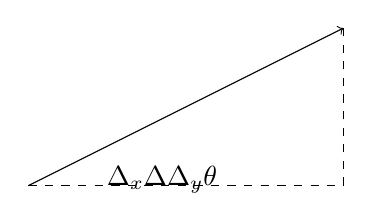
\begin{tikzpicture}
 
\coordinate (O) at (-1,0);
\coordinate (A) at (3,0);
\coordinate (B) at (3,2);
\draw[dashed] (O)--(A);
\draw[dashed] (A)--(B);
\draw[->] (O)--(B);

\tkzLabelSegment[below=1pt](O,A){$\Delta_x$}
\tkzLabelSegment[above=2pt](O,B){$\Delta$}
\tkzLabelSegment[right=2pt](A,B){$\Delta_y$}

\tkzMarkRightAngle[size=0.5,opacity=.4](O,A,B)% square angle here

\tkzLabelAngle[pos = 0.85](B,O,A){$\theta$}
\tkzMarkAngle[fill=gray, size=1.2cm, opacity=.4](A,O,B)


\end{tikzpicture}
\end{figure}